Las líneas de campo no son más que un medio para visualizar el patrón formado por el campo eléctrico a través del trazo de líneas conocidas como \textbf{líneas de campo eléctrico}. Estas líneas relacionan el campo eléctrico con una región del espacio de la siguiente manera:
\begin{itemize}
    \item El vector \(\vec{E}\) del campo eléctrico es tangente a la línea del campo eléctrico en cada punto y la dirección de la linea de campo es igual a la del campo eléctrico.
    \item El número de líneas de campo que pasan por una superficie perpendicular a dichas líneas es proporcional a la magnitud de campo.
\end{itemize}

\begin{figure}[ht]
    \centering
    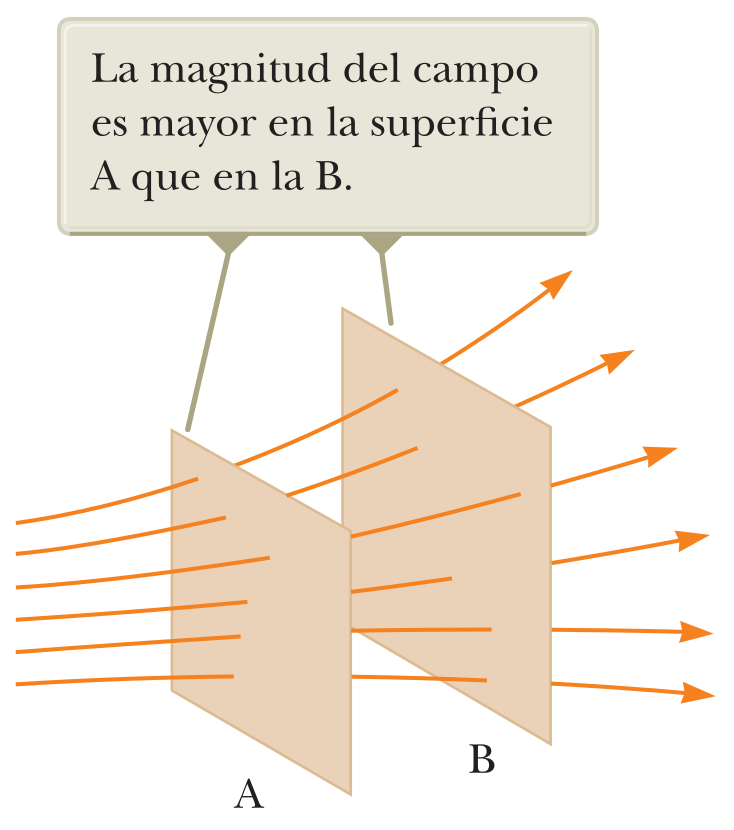
\includegraphics[width=0.5\textwidth]{field-lines.png}
    \caption{Líneas de campo eléctrico que atraviesan dos superficies}
    \label{fig:lineas_de_campo}
\end{figure}

Pongamos este concepto en palabras simples ¿Recuerdas el ejemplo de las tres cargas y el ``mapa de flechas''? Bueno, las líneas de campo nos ayudan a visualizar el ``mapa de flechas'' de una forma más cómoda.

\begin{figure}[ht]
    \centering
    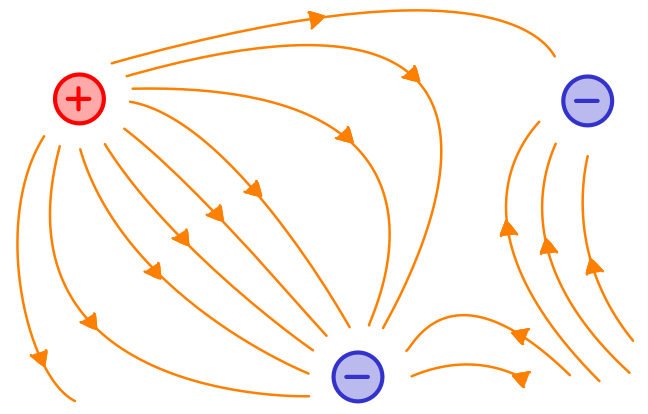
\includegraphics[width=0.4\textwidth]{field_lines_ex.png}
    \caption{Ejemplo del ``mapa de flechas'' visualizado con líneas de campo}
    \label{fig:ej_lineas_de_campo}
\end{figure}

En este caso se puede ver que las líneas de campo están más juntas cuando nos acercamos a las cargas, y se van separando cuando nos alejamos. La proximidad entre líneas de campo nos indica que el campo es intenso. Si las líneas están distantes entre sí indica que el campo es menos intenso. Esto se puede verificar con la ecuación del campo eléctrico, ya que el campo disminuye con el cuadrado de la distancia. Esto significa que según más nos alejamos de las cargas fuente, el campo disminuye.